\section{Core Hypotheses in Mechanistic Interpretability}
\label{sec:hypotheses}

Mechanistic interpretability rests on several core hypotheses about how neural networks represent information and implement computation. These hypotheses are not yet rigorously proven. Nonetheless, they have shaped methodological choices and empirical investigations. In this section, we formalise four of them, discuss their conceptual basis, and summarise supporting and opposing empirical evidence.

\subsection{The Linear Representation Hypothesis}
\label{subsec:linearity}

We have seen that single neurons may not be the most effective unit of representation in many cases, but what is? The linear representation hypothesis claims that \emph{linear} directions in the activation space are effective fundamental units of representation~\citeest{lrh}.


\begin{definitionbox}[Linear Representation Hypothesis]
A concept can be effectively represented by a feature corresponding to a linear direction $\phi$ in activation space $\mathbb{R}^d$. Linearity implies that adding or subtracting this direction, or a scalar multiple of it, from model activations can correspondingly influence model behaviour, while the projection $\phi^\top h(x)$ approximately measures the strength of the feature in model activations $h(x)$ for an input $x$.\\

Under a strong version of the linear representation hypothesis, all concepts are best represented by linear features. In this view, model activations can be approximately decomposed as an additive combination of such features,
\[
h(x) \approx \sum_i \alpha_i \phi_i,
\]
where $\alpha_i \in \mathbb{R}$ denotes the strength of feature $\phi_i$ dependent on the input $x$. Under a weaker version, only some concepts admit such linear representations~(\citeestalp{sharkey2025open}; \citeemalp{smith2024strongfeature}).
\end{definitionbox}

\paragraph{Conceptual Basis.} A feature associated with a concept is linearly represented if its presence corresponds to a fixed direction $\phi$ in the activation space and can be detected through the projection $\phi^\top h(x)$. This linearity makes mechanistic analysis tractable because we can use simple methods to identify, measure, and manipulate these features in the activation space, such as scaling them and adding them back to model activations.

Notably, activation spaces in different model components can have distinct geometric structures. For example, in the hidden states of MLP blocks, the neuron axes are computationally distinguished because element-wise nonlinear activation functions, such as ReLU, act separately on each axis. The coordinate system is therefore meaningful and is referred to as a \emph{privileged basis} (Figure~\ref{fig:privileged-basis}, left)~\citeem{elhage2022superposition}. In other spaces, such as the residual stream, no operation singles out the neuron axes, so linear features may lie along arbitrary directions. Such spaces are said to have a \emph{non-privileged basis} (Figure~\ref{fig:privileged-basis}, right).

\begin{figure}[tb]
  \centering
  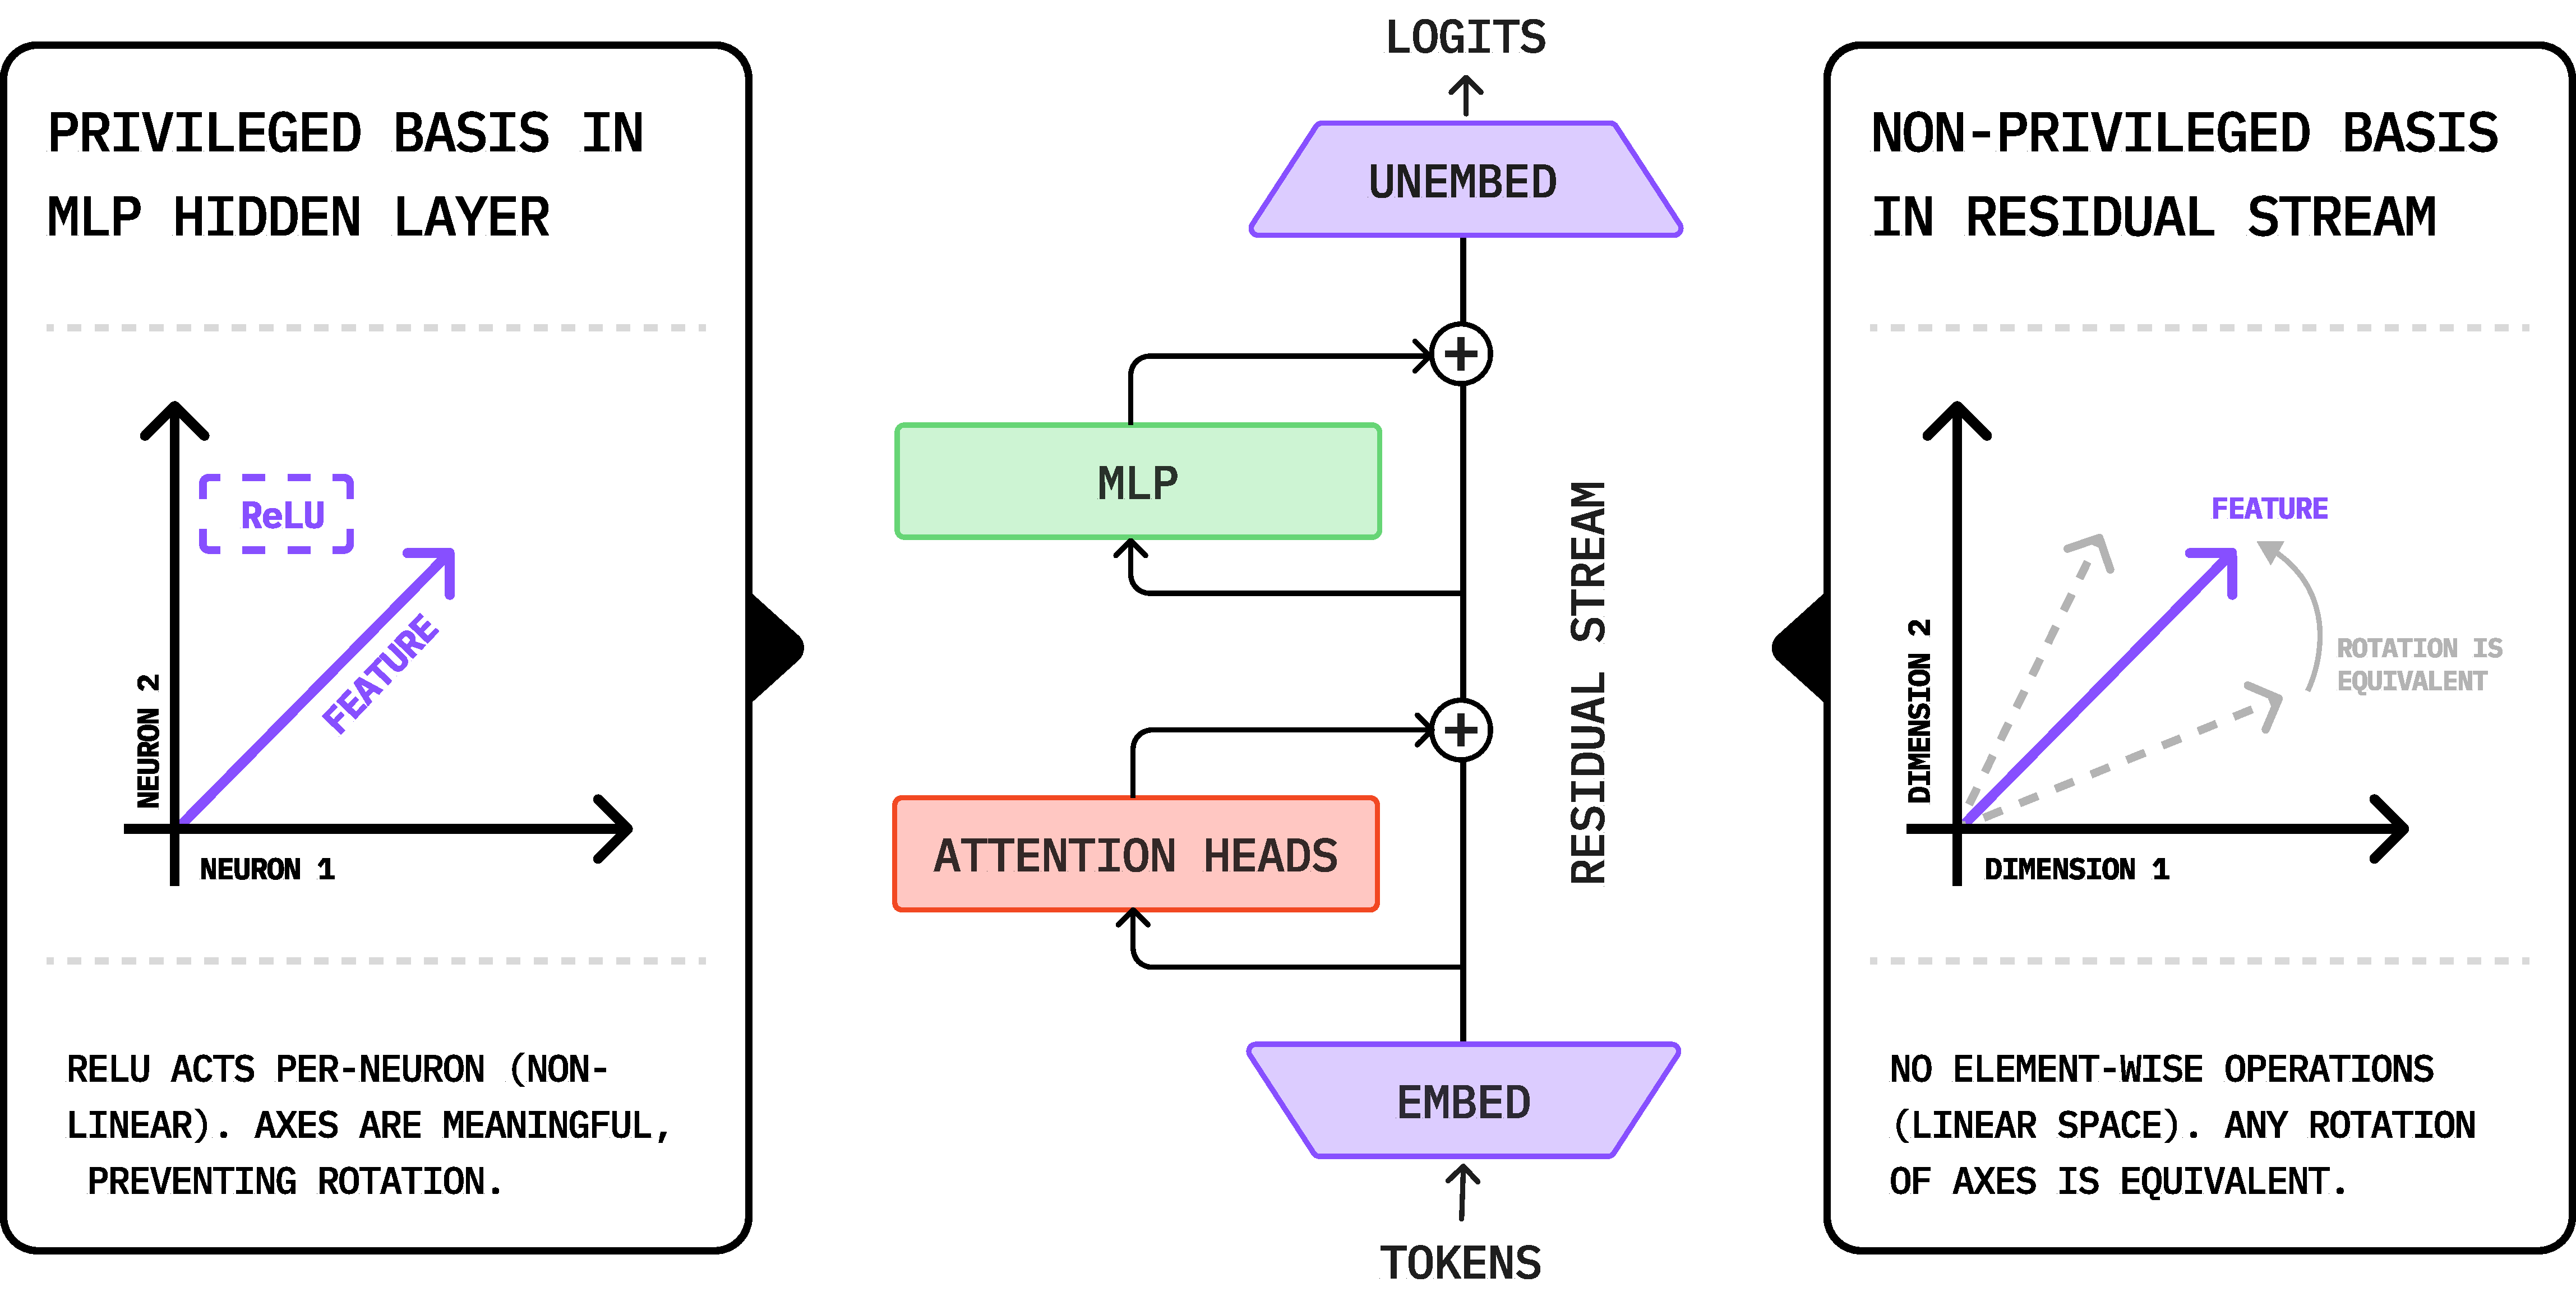
\includegraphics[width=\linewidth]{figs/5_Priviledge.pdf}
\caption{Privileged versus non-privileged bases. In the hidden layers of MLP blocks, element-wise nonlinear operations break rotational symmetry and make individual axes meaningful. In contrast, the residual stream contains no such operations that privilege particular axes, so rotating the basis preserves the relevant computation.}
  \label{fig:privileged-basis}
\end{figure}

When the basis is privileged, a single neuron can serve as a scalar feature that meaningfully represents a concept. When it is not, the feature may instead correspond to directions or other geometric structures that do not align with any individual neuron. In this case, specialised methods are required to identify them from the activation space.

\paragraph{Empirical Evidence and Counterexamples.}
Empirical support for the weaker version of the linear representation hypothesis includes the success of linear probes across diverse models and concepts~\citeest{belinkov-2022-probing}, activation steering along single directions to induce targeted behavioural changes~\citeem{turner2024steeringlanguagemodelsactivation}, and sparse autoencoders recovering linearly accessible and steerable features at scale~\citeem{bricken2023monosemanticity}. At the same time, there is substantial evidence that not all representations are well described as linear. Counterexamples include nonlinear feature interactions, algorithmic representations that rely on nonlinear transformations, and features distributed across multiple interacting subspaces~(\citeestalp{nanda2023progressmeasuresgrokkingmechanistic, engels2025languagemodelfeaturesonedimensionally, smds}; \citeemalp{rnnnonlinear, feucht2026arithmeticwildllamauses, wurgaft2026manifoldsteeringrevealsshared}). Some work has further argued that features may not always exist as explicitly represented objects, but may instead emerge from underlying circuit dynamics~\citeem{smith2024strongfeature}. The linear representation hypothesis is therefore best viewed as a useful approximation that holds in some settings, rather than as a universal law.

\subsection{The Superposition Hypothesis}
\label{subsec:superposition}

The superposition hypothesis says that models encode more features than their hidden representations have dimensions.

\begin{definitionbox}[Superposition Hypothesis]
Model hidden states encode more features than they have dimensions. If there are $m$ features and 
$d$ dimensions, then the superposition hypothesis claims that $m \gg d$.\\

This implies that features cannot be represented as orthogonal directions---though they can be represented as nearly orthogonal directions. It also implies neuron polysemanticity: the same neuron participates in the encoding of multiple unrelated concepts.
\end{definitionbox}

\paragraph{Conceptual Basis.}

Superposition is a geometric property of learned representations in which a limited number of neuron dimensions encode many more features by allowing those features to share representational dimensions. Neuron polysemanticity, where individual neurons respond to multiple seemingly unrelated semantic concepts, naturally follows from this phenomenon. When the number of encoded features exceeds the activation-space dimensionality, the model can no longer allocate a dedicated neuron dimension to each feature. Instead, multiple features become superposed within the same activation space, shifting the representation from dedicated dimensions with monosemantic neurons to shared dimensions with increasingly polysemantic neurons (Figure~\ref{fig:superposition-polysemanticity}).

\paragraph{Empirical Evidence.}
Mechanistic studies have repeatedly observed widespread neuron polysemanticity: individual neurons often activate for multiple seemingly unrelated semantic concepts, making them difficult to interpret as standalone representational units~\citeem{olah2020zoom, elhage2022superposition, bricken2023monosemanticity}. Dictionary-learning methods such as sparse autoencoders exploit this structure to recover millions of distinct features from shared activation spaces~\citeem{bricken2023monosemanticity, templeton2024scaling}. Many discovered features are substantially more monosemantic than individual neurons, and some have been shown to causally influence model behaviour. Together, these findings suggest that the activation space may encode more meaningful semantic information along activation-space directions than along individual neuron axes.

However, the superposition hypothesis remains a hypothesis, not an established fact, in large language models. Observing polysemantic neurons does not, by itself, imply that superposition is the underlying cause, and dictionary-learning methods can recover interpretable features even in the absence of superposition. Furthermore, \citetem{lecomte2024what} showed that polysemanticity can arise even when the number of underlying features does not exceed the number of available neurons, suggesting alternative---and potentially complementary---mechanisms for the emergence of polysemantic representations.

\begin{figure}[tb]
  \centering
  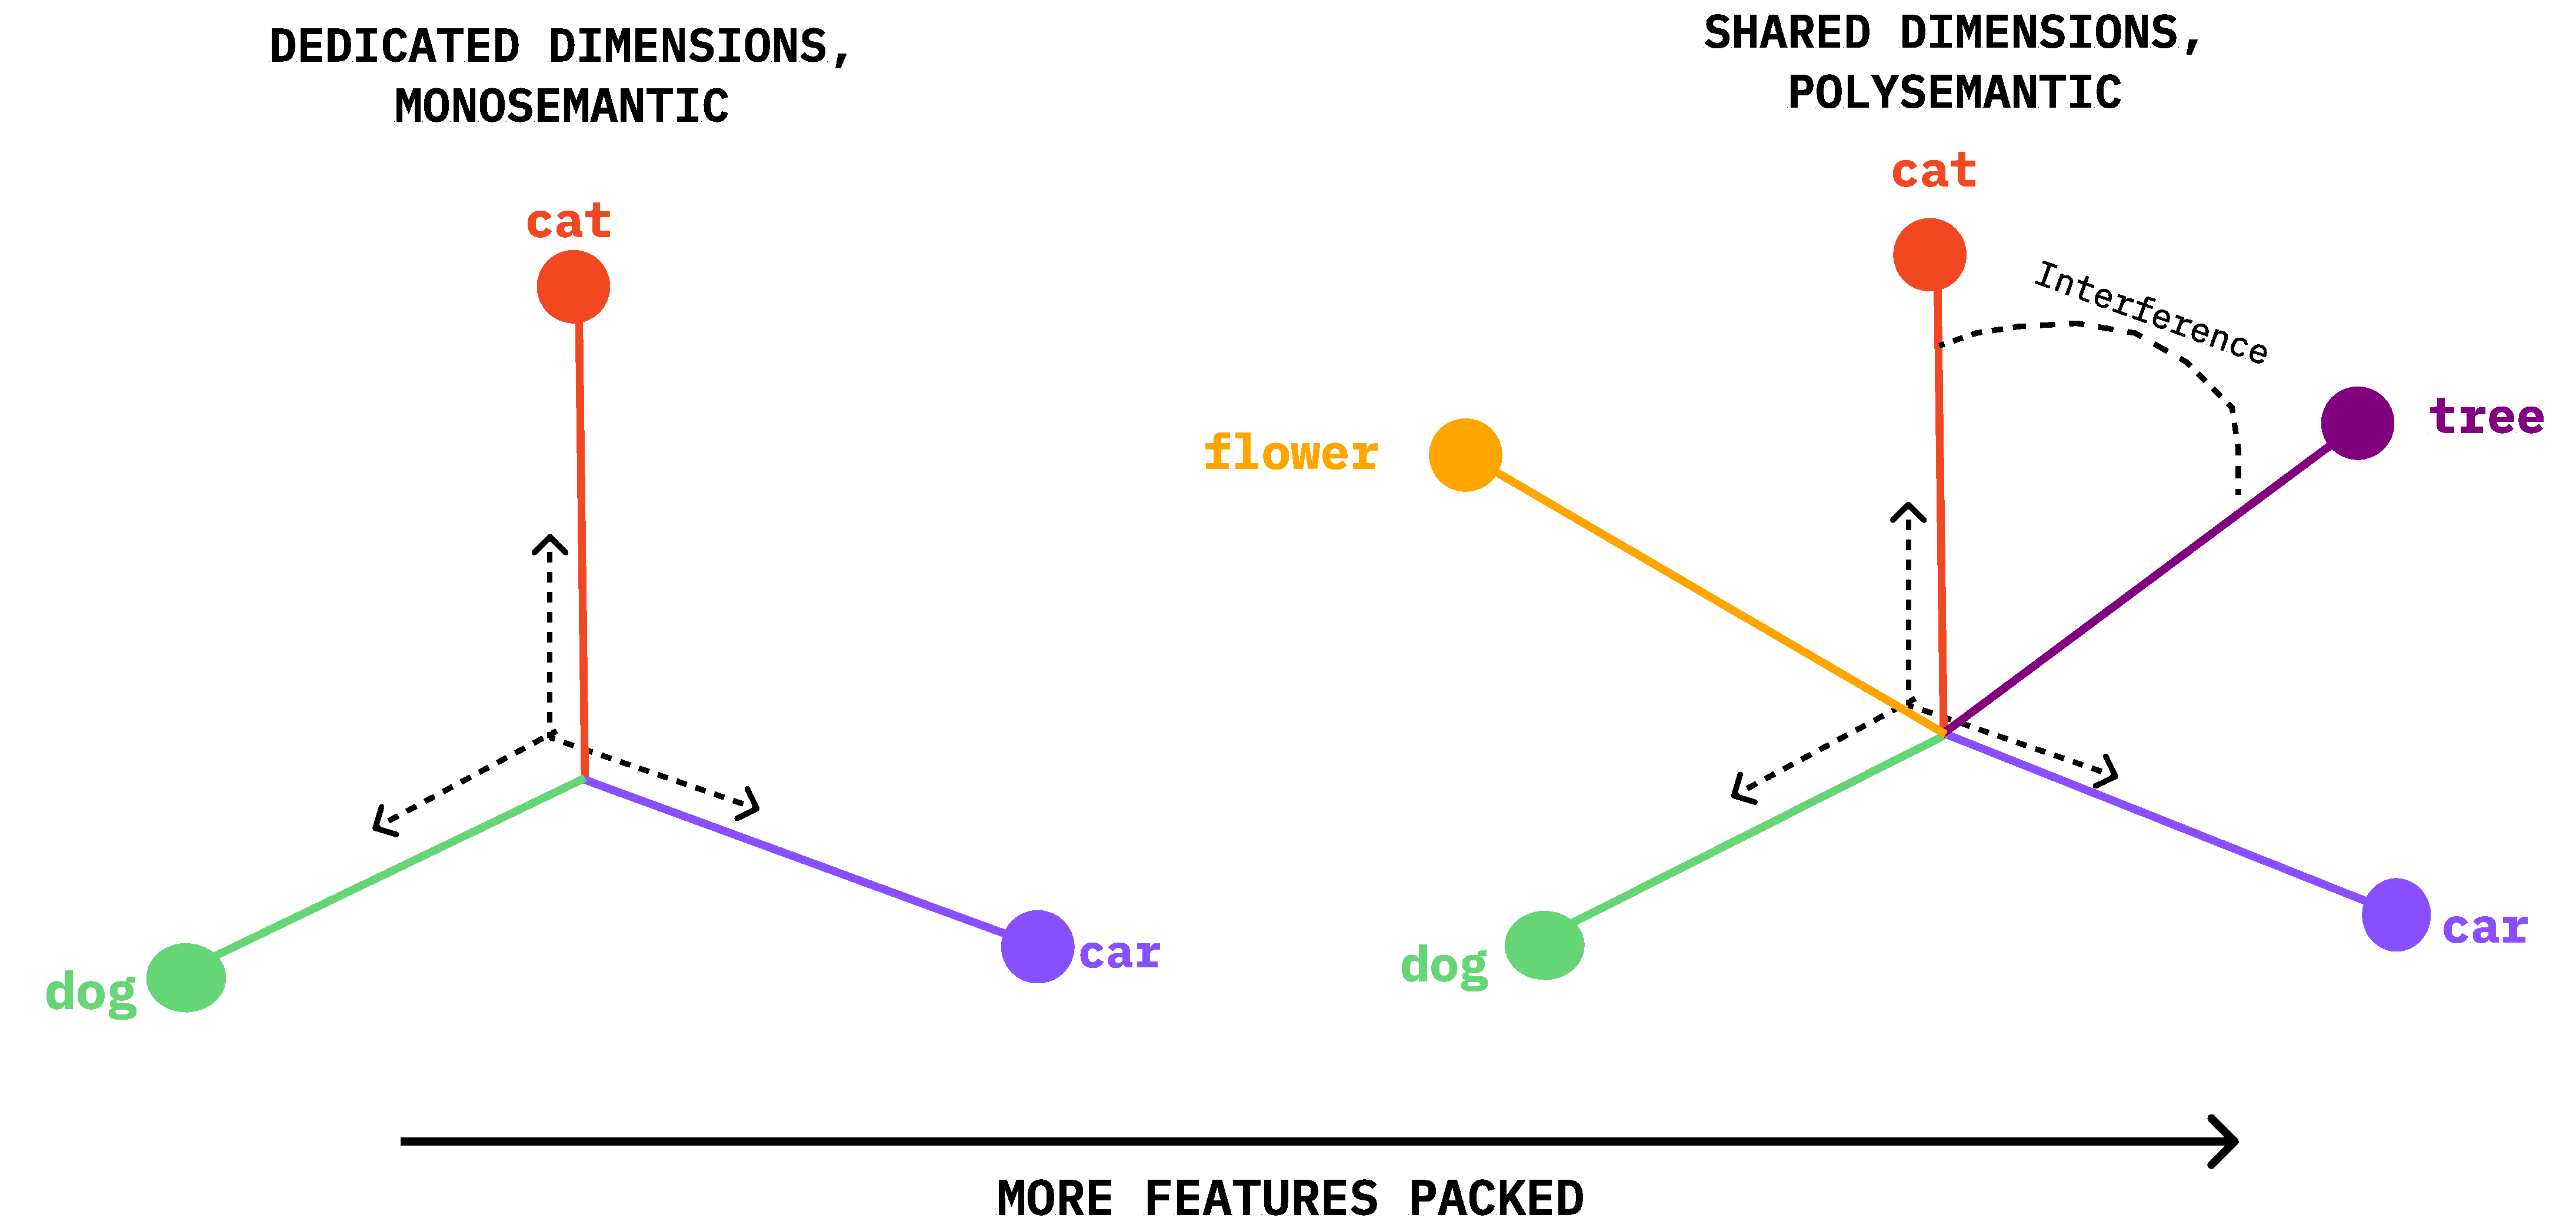
\includegraphics[width=\linewidth]{figs/5_Superposition_and_Polysemanticity.pdf}
  \caption{\textbf{Superposition implies polysemanticity.} Left: when the number of features $m$ does not exceed the number of dimensions $d$, i.e., $m\le d$, feature directions can align cleanly with individual neuron axes, producing monosemantic neurons. Right: when $m>d$, multiple feature directions must share the same limited set of neuron axes; as a result, each neuron axis cuts across multiple feature directions, producing polysemantic neurons.}
  \label{fig:superposition-polysemanticity}
\end{figure}

\paragraph{Architectural Responses to Superposition.} Superposition is not an intrinsically inevitable property of deep neural networks but a consequence of architectural permissiveness. Without constraints on model architectures or activations, gradient descent can exploit the activation-space geometry to pack far more features than neurons~\citeem{elhage2022superposition}. This motivates a distinct research direction, \emph{interpretability-by-design} (as mentioned in Section~\ref{subsec:cbm} and discussed in Section~\ref{sec:architectural-interventions}). Interpretability-by-design argues that, rather than decomposing traditional models' superposed activations post hoc, one can design novel architectures or components that encourage representations where features are more accessible for analysis. Two intervention points have been explored:

\begin{itemize}
    \item \textbf{Sparsity constraints:} Enforce sparsity in weights or activations that limits how many neurons within an MLP or attention head can participate for a given input, constraining how many units can jointly support any single feature~(\citeestalp{yang2025mixture, gao2025weight}; \citeemalp{elhage2022solu}).
    \item \textbf{Computational primitives:} Change the fundamental units of analysis from static features in activations to learnable transformations by weight matrices that generate activations~(\citeestalp{liu2025kan}; \citeemalp{anthropic2025molt}). This paradigm better matches certain tasks and avoids the pressure to compress or suppress model representations.
\end{itemize}

These architectural interventions shift from treating superposition as a phenomenon to reverse-engineer to treating it as a design choice that can be constrained upstream. We discuss these methods in detail in Section~\ref{sec:architectural-interventions}.

\subsection{The Privileged Access Hypothesis} 
\label{subsec:privileged-access}
A class of approaches that use language models as interpreters of \textit{themselves} can be justified through the privileged access hypothesis. The privileged access hypothesis states that:
\begin{definitionbox}[Privileged Access Hypothesis]
A language model used to interpret itself can, under appropriate elicitation, access internal variables and intermediate computations that are not reliably recoverable from external behavioural analysis alone, providing a comparative advantage as an interpreter of its own behaviour~(\citeestalp{binder}; \citeemalp{li2025traininglanguagemodelsexplain, song}).
\end{definitionbox}

\paragraph{Conceptual Basis.} The ability to access and judge its own computation or reasoning---called \emph{introspective monitoring}---has long been a desired property of an AI system~\citeem{cox2008metareasoning}. Even earlier rule-based medical expert systems sought to explain their decisions, such as MYCIN's ``Explanation system''~\citeest{shortliffe1977mycin}. In this sense, using language models to explain themselves can be seen as a modern continuation of these earlier efforts.

A major difference is that rule-based systems can explicitly present the rule they executed, whereas modern language models compute in a highly nonlinear way. Although researchers have proposed mechanistic tools aiming to reverse-engineer part of the computation, the technical complexity of these techniques hinders their accessibility and scalability. The privileged access hypothesis then posits that the language model itself naturally stores information about the computation within its internal states, such as latent beliefs or intermediate plans. The model can thus learn to verbalise this information directly, serving as a scalable complement to mechanistic analysis.

\paragraph{Empirical Evidence.}



The most direct empirical evidence for this hypothesis comes from recent findings that models, even without explicit training to do so, are sometimes aware of concept representations (acquired by methods like difference-in-means) injected into their activations~\citeem{lindsey2026emergentintrospectiveawarenesslarge, fornasiere2026languagemodelsrecognizedropout}. Additional, though less direct, evidence comes from the design of explainer models---a general class of interpretability methods in which one model is fine-tuned to explain the target model’s activations~(\citeestalp{pan2024latentqateachingllmsdecode, ao}; \citeemalp{nla}). In practice, such explainers are typically initialised from a copy of the target model itself~(\citeestalp{pan2024latentqateachingllmsdecode, ao}; \citeemalp{buildingbetterao, pcd}). This usually works better than initialising from alternative models, suggesting the target model already encodes much of what is needed to interpret its own activations. In this sense, fine-tuning elicits and refines a latent capability rather than creating one from scratch.


Some studies also reported negative results for the privileged access hypothesis: \citetem{song} found that models predict their own sampling temperature no better than they predict other models', suggesting apparent introspection may reflect general reasoning about model-like systems rather than self-access. Separately, recent work has questioned whether internals-based explanations provide a practical advantage over behavioural baselines: \citetem{chive} found that activation-reading tools (including activation oracles) give agents no uplift over transcript-only baselines at predicting counterfactual model behaviours in the wild, and \citetest{li2026do} showed that standard verbalisation benchmarks can be solved without access to target-model internals at all~(see also \citeemalp{jakkli2026current}).

In summary, these results show that privileged access is \textit{possible} for certain tasks under favourable conditions, not \textit{universal} or \textit{reliable}. The hypothesis should therefore be treated with caution, as significant failure modes and limitations remain.





\subsection{The Universality and Platonic Representation Hypothesis}
\label{subsec:universality}

\begin{definitionbox}[Platonic Representation Hypothesis]
Models independently trained on similar tasks tend to develop similar internal representations or algorithms, which often approximate a task-determined canonical form (\citeestalp{huh2024platonicrepresentationhypothesis}; \citeemalp{olah2020zoom}). The degree of convergence depends on factors such as model size, architecture, and training data.
\end{definitionbox}

\paragraph{Conceptual Basis.}
A key distinction is the level at which models are expected to converge. \emph{Weak universality} refers to convergence in the algorithms or recurring computational patterns that models implement, even when these are encoded through different internal representations. \emph{Strong universality} makes the stronger claim that the internal representations themselves converge towards a shared canonical form.

\paragraph{Empirical Evidence and Trade-Offs.}
Weak universality is supported by recurring attention patterns, features, and circuits across models, tasks, and scales~(\citeestalp{nanda2023progressmeasuresgrokkingmechanistic, lan-etal-2024-towards}; \citeemalp{olah2020zoom, quirke2026understandingadditionsubtractiontransformers}). Strong universality is less supported and is usually demonstrated through representational similarity metrics~(\citeestalp{kornblith2019similarityneuralnetworkrepresentations, moschella2023relative}; \citeemalp{lan2025quantifyingfeaturespaceuniversality}), where recent studies have found the results to be fragile~(\citeestalp{groger2026revisiting}; \citeemalp{koepke2026platoscaveexaminingcrossmodal}). Divergent representations can arise from variations in architecture, data, or optimisation trajectories~\citeest{harrasse2025tinysqlprogressivetexttosqldataset, morcos2018insightsrepresentationalsimilarityneural}.

\paragraph{Implications.}
If strong universality holds, fine-grained mechanistic insights and the methods derived from them may transfer more readily across models. If only weak universality holds, such insights may remain contingent on factors such as model family and task~\citeest{bereska2024mechanisticinterpretabilityaisafety}, and even a complete mechanistic understanding of one model (see Section~\ref{subsec:ambitious}) may fail to generalise to others. Therefore, it is important to clarify the extent of universality for assessing the promise, limitations, and scalability of different interpretability research orientations, including the six major orientations introduced in Section~\ref{sec:orientations}.

\paragraph{Summary.} This section discussed four hypotheses that motivate many modern mechanistic interpretability studies. Linear representations support linear-feature-based analysis; superposition explains why we need to operate on linear or more complex forms of features instead of single neurons; privileged access explains the fundamental idea of model self-interpretation; universality asks whether insights transfer across models and at which levels. Each hypothesis holds in some settings and fails in others, and techniques built on them inherit those limitations. Section~\ref{sec:sae} introduces the main family of techniques and methods that operationalise the first two hypotheses (linear representation and superposition): dictionary learning for feature extraction and analysis.
